%======================================================================
\chapter{Implementation}
\label{ch: Chapter5}
%======================================================================

%----------------------------------------------------------------------
\section{Robot Assembly}
%----------------------------------------------------------------------

For this project we needed a Remote Target and Smart Robotic Cart that we designed and implemented from off the shelf components.  As mentioned above in \autoref{sec:System Components} some of our components came from what the school already owned as well as some we had to buy specifically for this project listed in \autoref{tab:Partslablist} and \autoref{tab:Partslablist}.\par
Since the school already owned the Budget Bot chassis, we opted to use these base cart chassis frames to build our Smart Robotic Cart upon.  The base Budget Bot chassis did need to be modified slightly to work with our project.  The main change was that we swapped out the motors that came with the Budget Bot for Pololu 27D Meatal Gear motors since the original motors spin at max speed is 212 RPM or 1.09m/s and the new motors max speed is 530 RPM or 2.72m/s when using the base wheels that have a diameter of 98mm.  By switching out the motors we are able to achieve our goal of  matching an average person's walking speed of 1.5m/s since the build in motors can not achieve this. The other modifications to the chassis are that a hard power switch was added to directly cut off power to the XBee modules in the reflector as well as a power indicator LED. \par

\begin{figure}
	\centering
	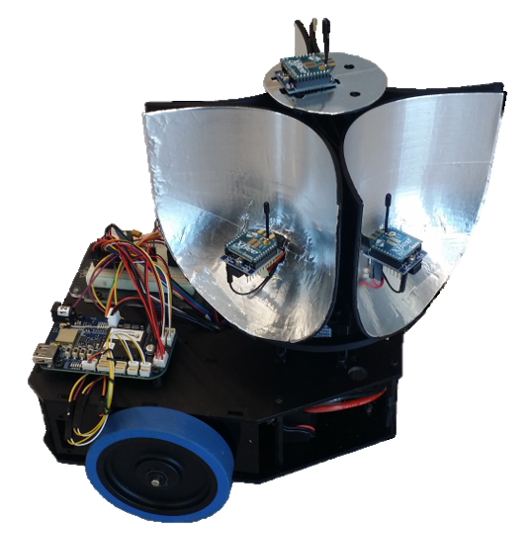
\includegraphics[width=0.5\textwidth]{figs/img/Finalized_robot.png}
	\caption{Final Version of the Robotic Cart}
 	\label{fig:FinalizedRobot}
\end{figure}

As can be seen in \autoref{fig:FinalizedRobot} our next step was to attach the Beagle Bone Blue microcomputer, XBee reflector array assembly, and breadboard to the top of the robot.  We also installed a 2-cell LiPo battery inside the body of the mobile cart that delivers power to the Beagle Bone Blue directly and power to the breadboard through the switch. \par
The power supplied to the breadboard is sent through a regulator circuit to drop it down from 7.4v from the LiPo to 3.3v.  This same circuit also is used on the remote which consists only of a 9v battery and the XBee module with this voltage regulator in between.  This voltage regulator is build out of a LM117 regulator and a 10uF ceramic capacitor between the input and output pins of the regulator as shown in \autoref{fig:PowerConverter}.

\begin{figure}
	\centering
	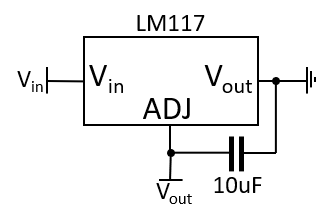
\includegraphics[width=0.5\textwidth]{figs/img/PowerConverter.png}
	\caption{Final Version of the Robotic Cart}
 	\label{fig:PowerConverter}
\end{figure}

The Reflector array assembly from \autoref{ch: Chapter3} was mounted on a stepper motor that was then attached to the robot chasse using a 3D printed bracket.  This bracket was the attached to the chasse using bolts.  Another feature of this bracket is that it had a stop block built into the top of it that is used to automatically zero the reflector array when the robot starts up.\par
The Xbee modules from the reflector posed a bit of a problem when it came to connecting them to the Beagle Bone Blue.  This problem comes from that the Beagle Bone Blue has five UART ports if we are using the one found in the USB and the UART-GPS along with the three normal UART ports.  This unfortunately dose not work though since UART port zero is tied to the council used to communicate with it from a computer.  Since this port is reserved for this function that reduces the number of usable ports down to four which does not work since we have five XBees in it.  Our solution to this was to use two of the GPIO pins, two of the UART ports, and a two-way multiplexer.  With this setup we can directly connect one of the UARTs to the top XBee and then rout the other four side XBee modules through the MUX so only one UART port is needed for them.


%----------------------------------------------------------------------
\section{Code Base}
%----------------------------------------------------------------------

\todo[inline]{Please complete this section}

%----------------------------------------------------------------------
\section{Algorithm Testing}
%----------------------------------------------------------------------



%----------------------------------------------------------------------
\section{Experimental Results}
%----------------------------------------------------------------------

\todo[inline]{See page 23 of~\url{http://ee.bradley.edu/projects/proj2017/ekf_slam/Downloads/seniorProject_finalReport.pdf}}


\section{Simulation using Robot Simulator}

\todo[inline]{In this section, we detail the steps of simulating the proposed
  robotic cart using a commercial robot simulator CoppeliaSim. $\ldots \ldots$}


%%% Local Variables:
%%% mode: latex
%%% TeX-master: "../finalReport"
%%% End:
